\documentclass[10pt, a5paper]{article}
\usepackage{pdfpages}
\usepackage{parallel}
\usepackage[T2A]{fontenc}
\usepackage{ucs}
\usepackage[utf8x]{inputenc}
\usepackage[polish,english,russian]{babel}
\usepackage{hyperref}
\usepackage{rotating}
\usepackage[inner=2cm,top=1.8cm,outer=2cm,bottom=2.3cm,nohead]{geometry}
\usepackage{listings}
\usepackage{graphicx}
\usepackage{wrapfig}
\usepackage{longtable}
\usepackage{indentfirst}
\usepackage{array}
\newcolumntype{P}[1]{>{\raggedright\arraybackslash}p{#1}}
\frenchspacing
\usepackage{fixltx2e} %text sub- and superscripts
\usepackage{icomma} % коскі ў матэматычным рэжыме
\PreloadUnicodePage{4}

\newcommand{\longpage}{\enlargethispage{\baselineskip}}
\newcommand{\shortpage}{\enlargethispage{-\baselineskip}}

\def\switchlang#1{\expandafter\csname switchlang#1\endcsname}
\def\switchlangbe{
\let\saverefname=\refname%
\def\refname{Літаратура}%
\def\figurename{Іл.}%
}
\def\switchlangen{
\let\saverefname=\refname%
\def\refname{References}%
\def\figurename{Fig.}%
}
\def\switchlangru{
\let\saverefname=\refname%
\let\savefigurename=\figurename%
\def\refname{Литература}%
\def\figurename{Рис.}%
}

\hyphenation{admi-ni-stra-tive}
\hyphenation{ex-pe-ri-ence}
\hyphenation{fle-xi-bi-li-ty}
\hyphenation{Py-thon}
\hyphenation{ma-the-ma-ti-cal}
\hyphenation{re-ported}
\hyphenation{imp-le-menta-tions}
\hyphenation{pro-vides}
\hyphenation{en-gi-neering}
\hyphenation{com-pa-ti-bi-li-ty}
\hyphenation{im-pos-sible}
\hyphenation{desk-top}
\hyphenation{elec-tro-nic}
\hyphenation{com-pa-ny}
\hyphenation{de-ve-lop-ment}
\hyphenation{de-ve-loping}
\hyphenation{de-ve-lop}
\hyphenation{da-ta-ba-se}
\hyphenation{plat-forms}
\hyphenation{or-ga-ni-za-tion}
\hyphenation{pro-gramming}
\hyphenation{in-stru-ments}
\hyphenation{Li-nux}
\hyphenation{sour-ce}
\hyphenation{en-vi-ron-ment}
\hyphenation{Te-le-pathy}
\hyphenation{Li-nux-ov-ka}
\hyphenation{Open-BSD}
\hyphenation{Free-BSD}
\hyphenation{men-ti-on-ed}
\hyphenation{app-li-ca-tion}

\def\progref!#1!{\texttt{#1}}
\renewcommand{\arraystretch}{2} %Іначай формулы ў матрыцы зліпаюцца з лініямі
\usepackage{array}

\def\interview #1 (#2), #3, #4, #5\par{

\section[#1, #3, #4]{#1 -- #3, #4}
\def\qname{LVEE}
\def\aname{#1}
\def\q ##1\par{{\noindent \bf \qname: ##1 }\par}
\def\a{{\noindent \bf \aname: } \def\qname{L}\def\aname{#2}}
}

\def\interview* #1 (#2), #3, #4, #5\par{

\section*{#1\\{\small\rm #3, #4. #5}}

\def\qname{LVEE}
\def\aname{#1}
\def\q ##1\par{{\noindent \bf \qname: ##1 }\par}
\def\a{{\noindent \bf \aname: } \def\qname{L}\def\aname{#2}}
}

\begin{document}
\switchlang{en}
\title{Berkeley Open Infrastructure for Network Computing — an open distributed computing system}
\author{\L{}ukasz \'{S}wierczewski\footnote{\L{}om\.z{}a, Poland; \url{lswierczewski@pwsip.edu.pl}}}
\maketitle
Each year, the demand on computing resources of scientific and military institutions is increasing significantly. This process is noticeable almost from the very beginning of computers, which were quickly\linebreak harnessed to complicated calculations. The symbol of advanced \linebreak technology is TOP500 list. Updated twice a year, ranking presents 500 fastest computers on Earth.

\begin{figure}[h!]
  \centering
  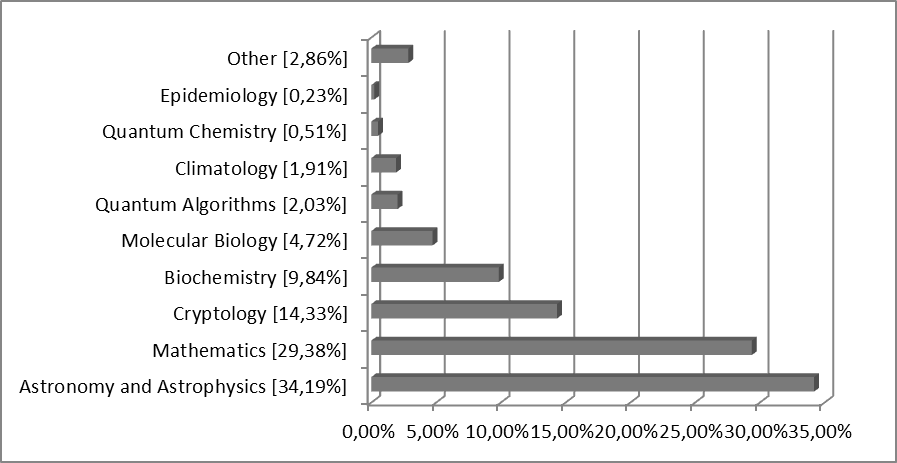
\includegraphics[width=10cm]{104_2013_w_Swierczewski_boinc_1}
  \caption{The division of all credits granted by BOINC in terms of scientific disciplines which concern the calculation.}\label{fig:swier1}
\end{figure}

An interesting alternative to centralized supercomputers is BOINC. BOINC (\cite{swier1}) is a system enabling use of personal computers for scientific research, and so, it can be considered as the the way to crowdsource scientific calculations. It allows to carry out calculations on a large scale incurring minimal costs associated with the purchase of equipment and its operation. In the case of BOINC infrastructure, as administrators we are forced to take care only of servers, which send computing tasks to the computers of individuals who have agreed to use their machines in his spare time to performed calculations for the good of science.

The user attaching to BOINC can choose one or several projects, in which he or she wishes to participate. The choice is very wide and covers many scientific fields from the mathematics and astrophysics to biochemistry. List of the best-known projects includes, among others, World Community Grid (\cite{swier2}). WCG is funded and managed by IBM. By providing the computing power of your PC in this project it contributes into, for example, the development of AIDS research, or into search of treatment for schistosomiasis. The LHC@Home (\cite{swier3}), which supports the project Large Hadron Collider (LHC), is also worth mentioning. One of the CERN department  decided to use BOINC to simulate the behavior of particles orbiting in the accelerator which allows to study the stability of their trajectory. During the test on each machine simulates the most common trip 60 particles around the ring by 100 000 laps.

\begin{figure}[h]
  \centering
  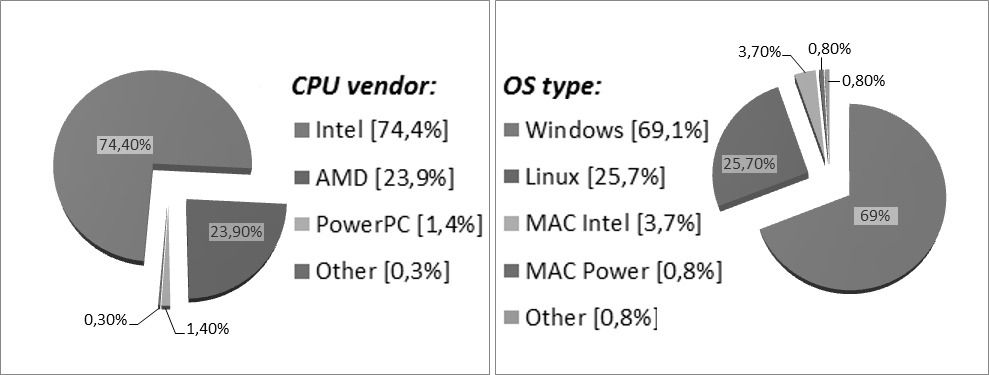
\includegraphics[width=10cm]{104_2013_w_Swierczewski_boinc_2}
  \caption{Operating systems and processors of the BOINC users.}\label{fig:swier2}
\end{figure}


After registration, the BOINC and calculated in the selected pro\-ject's first tasks, you will receive points. They are to some extent paid for their input in the development of science.
Number of points owned by the user should reflect how much time user's computers are dedicated to solving computational tasks. Fig.~\ref{fig:swier1} presents the percentage of all points in the various fields of science. It is seen, that projects for Astronomy and Astrophysics are the most popular ones. Second place belongs to the queen of sciences, i.e. to mathematics. Distribution of points over  nationalities is a special subject of interest. First position in terms of participation in BOINC belongs to Americans, of course, who have a significant advantage over Germans. The top five includes also England, Japan and France. This comparison is presented in Fig.~\ref{fig:swier3}. Fig.~\ref{fig:swier2} presents a summary on used processors and operating systems. Linux operating system has a relatively large group of users here "--- up to 25.70\%.

\begin{figure}[h]
  \centering
  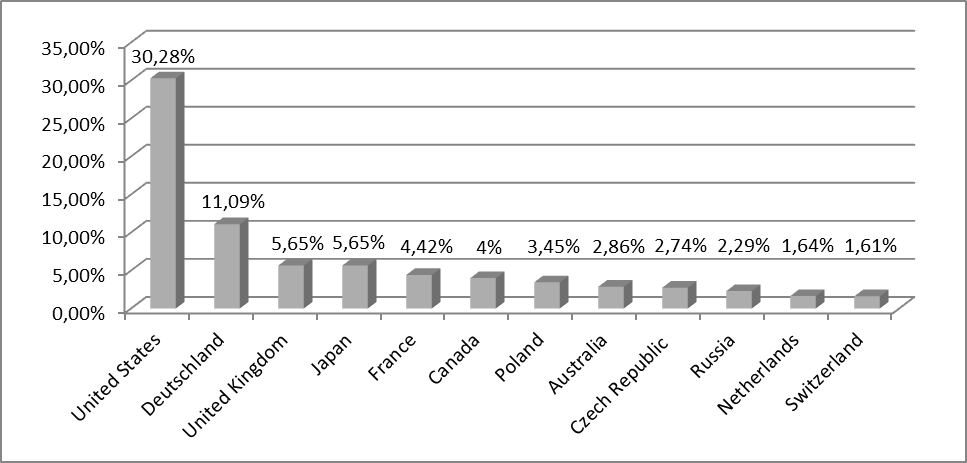
\includegraphics[width=10cm]{104_2013_w_Swierczewski_boinc_3}
  \caption{The country ranking in terms of quantity calculations carried out by members of the appropriate nationality.}\label{fig:swier3}
\end{figure}

Certainly it can be concluded that BOINC platform as a solution is worth of attention even for those who have no connection with science.

With this kind of initiatives we can make something significant for our common civilization.

\begin{thebibliography}{9}
\bibitem{swier1} BOINC homepage: \url{http://boinc.berkeley.edu/}
\bibitem{swier2} World Community Grid website: \url{http://www.worldcommunitygrid.org/}
\bibitem{swier3} LHC@Home website: \url{http://lhcathome.web.cern.ch/LHCathome/}
\end{thebibliography}

\end{document}
